Eine unit\"are Matrix besitzt einen oder mehere Eigenvektoren $|\psi\rangle$ mit zugeh\"origen Eigenwerten $e^{2\pi i \theta}$.
\begin{equation}
\label{eqn:eigenwert}
  U|\psi\rangle = e^{2\pi i \theta}|\psi\rangle
\end{equation}
Die Quantenphasensch\"atzung \textit{(quantum phase estimation)} kann die Phase $\theta$ aus Gleichung \ref{eqn:eigenwert} bestimmen. Dies gilt unter der Bedingung, dass diese Phase die eines Eigenwertes ist. D.h. der Zustand $|\psi\rangle$ muss so angepsasst sein, dass er ein Eigenzustand von $U$ ist. Es kann somit Phasenr\"uckschlag \textit{(Phasekickback)} und das wiederholte Ausf\"uhren von $U$ genutzt werden, um die Phase von $U$ in $\theta$ zu schreiben. Diese Phase kann mittles inverser QFT aus seinem Fourierzustand zu einem Basiszustand gewandelt werden. Die Schaltung der Quantenphasensch\"atzung (Abbildung \ref{fig:QPE}) wird auf zwei Quantenresgistern angewandt und wird aus zwei Teilen zusammengestellt. Das erste Quantenregister besteht aus $t$ Qubits die alle mit dem Basiszustand $|0\rangle$ initialisiert werden. Die Anzahl an Qubits f\"ur dieses Register wird nach der gew\"unschten Genauigkeit f\"ur die Sch\"atzung der Phase abh\"angig gemacht. Je gr\"o\ss er $t$ gew\"ahlt wird, desto gr\"o\ss er ist die Anzahl an Ziffern f\"ur die Sch\"atzung und auch die Wahrscheinlichkeit, dass die Phasensch\"atzung erfolgreich ist.
\begin{figure}[h]
  \centering
  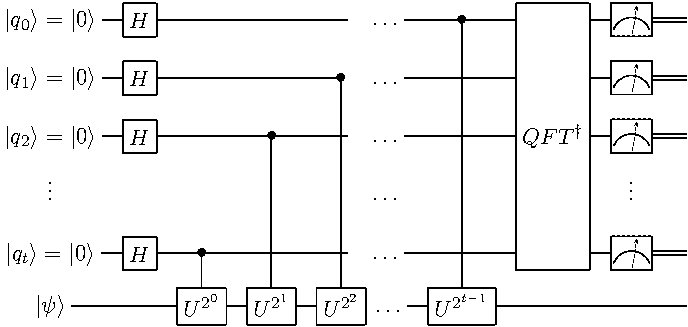
\includegraphics[width=1\textwidth]{figures/QPE.pdf}
  \caption{Allgemeine Schaltung der Quantenphasensch\"atzung (vgl. \cite{nielsen_chuang_2010})}
  \label{fig:QPE}
\end{figure}
Das zweite Quantenregister ist der Eigenvektor $|\psi\rangle$, f\"ur dieses Register werden so viele Qubits genutzt wie f\"ur die Darstellung des Zustands ben\"otigt werden.\\\\
Im ersten Teil der Schaltung wird auf allen Qubits aus dem ersten Register eine Hadamard-Transformation ausgef\"uhrt. Daraufhin wird eine kontrollierte $U$-Transformation auf das zweite Register ausgef\"uhrt, bei diesem $U$-Gatter erh\"oht sich wie ersichtlich stetig die 2er Potenz. Im zweiten Teil der Schaltung wird auf das erste Register eine invertierte Quantum Fourier-Transformation angewandt. \cite{Qiskit-Textbook} zeigt detaillierter wie das erste Register durch die Schaltung in folgenden Zustand ger\"at \ref{eqn:QPE}.
\begin{equation}
  \label{eqn:QPE}
  \begin{aligned}
    \frac{1}{\sqrt{2^t}}\sum\limits_{k=0}^{2^t-1}e^{2\pi i\theta k}|k\rangle = &\frac{1}{\sqrt{2^t}} \left(|0\rangle+e^{2\pi i 2^{t-1}\theta}|1\rangle\right)\otimes \\
    &\left(|0\rangle+e^{2\pi i 2^{t-2}\theta}|1\rangle\right)\otimes\dots\otimes\left(|0\rangle+e^{2\pi i 2^{0}\theta}|1\rangle\right).
  \end{aligned}
\end{equation}
In Anhang \ref{chap:anhang} Listing \ref{list:qpe} wird die Implementierung der Quantenphasensch\"atzung f\"ur die unit\"are Operation $P(\phi = \frac{\pi}{2})$ mit einem Quantenregister von $t = 3$ gezeigt. Das aus dieser Messung erhaltene Ergebnis muss durch $2^t$ geteilt werden um die Phase $\theta$ zu erhalten.
